\scanpage{44}

Genre de la courbe de Fermat $C_n$ (qui est une courbe \deleted{\unsure{projective}}\inserted{plane} lisse de degré $n$)

\[
g_n=\frac{(n-1)(n-2)}{2}
\]

le genre est $0$ \unsure{sss|ssi} $n=1,2$, il est $1$ sss $n=3$. Pour $n=4$ il est $3$, pour $n=6$ il est $10$, pour $n=12$ il est $55$ .....

\centerline{\rule{4em}{0.4pt}}
Considérons le cas $n=2$

\[
C_2:\quad x^2+y^2+z^2=0
\]

comme carte triangulée pondérée elle est formée de $4.2=8$ triangles, chaque type de sommet intervient $2$ fois, avec degré $4$ \inserted{($=2.2$)} \unsure{pour des gens au courant.|pour degré en un vert.|pour les gens au courant.} Sauf erreur, c'est l'\uline{\unsure{octoèdre|octaèdre}} \inserted{sphérique}, dont le groupe des automorphismes orientés est bien \inserted{$\simeq$}$\unsure{\mathfrak S_4|\mathscr S_4}$ d'ordre $24$, et peut s'écrire comme produit $1/2$ direct de $\mathfrak S_3$ par $(\mathbb Z_2)^2$ !

\figure{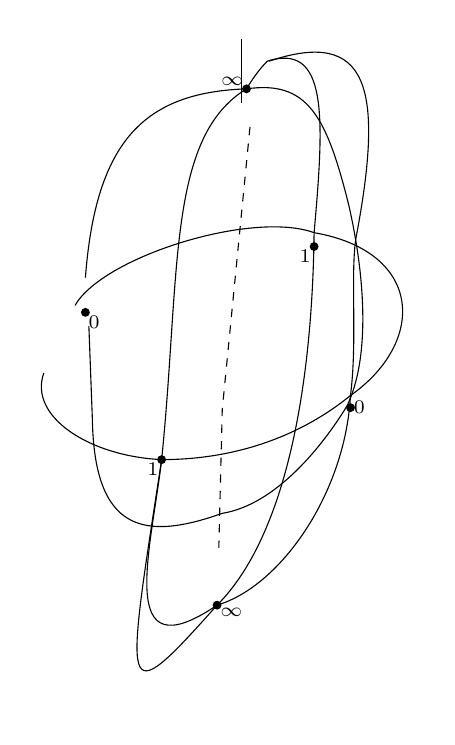
\begin{tikzpicture}[x=.022cm,y=-.022cm,every node/.style={font=\scriptsize,inner sep=1pt}]
\draw (120,5)--(120,42);
\draw (30,143) .. controls (36,64) and (64,36) .. (123,34) .. controls (158,29) and (169,49) .. (182,101) .. controls (192,145) and (194,190) .. (181,217) .. controls (167,240) and (140,274) .. (109,279) .. controls (64,295) and (35,290) .. (34,224) -- (32,171);
\draw (24,159) .. controls (40,131) and (126,104) .. (162,117) .. controls (225,128) and (227,180) .. (183,211) .. controls (156,233) and (119,248) .. (74,248) .. controls (32,246) and (-3,223) .. (6,198);
\draw (123,34) .. controls (77,62) and (85,140) .. (74,248) .. controls (68,300) and (47,372) .. (106,332) .. controls (146,292) and (161,205) .. (162,117) .. controls (168,50) and (170,7) .. (135,18) .. controls (130,23) and (126,29) .. (123,34);
\draw (136,18) .. controls (193,-1) and (203,32) .. (186,121) .. controls (183,143) and (187,180) .. (183,211) .. controls (180,267) and (143,321) .. (106,332) .. controls (49,396) and (53,386) .. (74,248);
\draw[dashed,thin] (125,56)--(109,219)--(107,299);
\fill (123,34) circle(1.6pt) node[above left] {$\infty$};
\fill (30,163) circle(1.6pt) node[below right] {$0$};
\fill (162,125) circle(1.6pt) node[below left] {$1$};
\fill (183,218) circle(1.6pt) node[right] {$0$};
\fill (74,248) circle(1.6pt) node[below left] {$1$};
\fill (106,332) circle(1.6pt) node[below right] {$\infty$};
\end{tikzpicture}}

Divisant par les trois ss-gpes $\mathbb F_2$ de $\Pi_2\simeq\mu_2^3/\mu_2$, on trouve les \inserted{$3$} revêtements d'ordre $2$ de $C_1\simeq\mathbb P^1_{\mathbb Q}$ qui correspondent au \deleted{dièdre}\inserted{monoèdre} \deleted{\unsure{pointés}} (autodual) et à ses transformés par $\mathfrak S_3$

\margin{\uline{NB} L'octaèdre est subdivision barycentrique du bi-èdre (qui est autodual) et a le type de ramification}

\figure{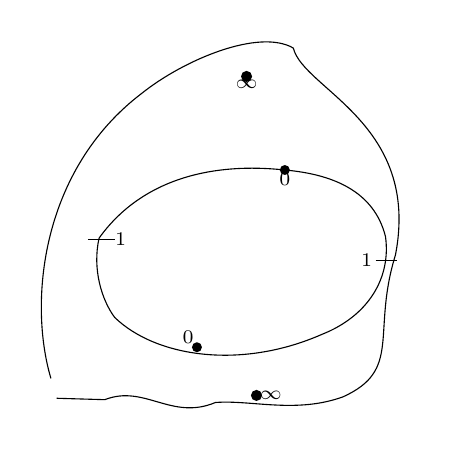
\begin{tikzpicture}[x=.018cm,y=-.018cm,every node/.style={font=\scriptsize,inner sep=1pt}]
\draw (3,238) .. controls (-13,184) and (-4,91) .. (67,37) .. controls (97,13) and (150,-9) .. (174,5) .. controls (181,34) and (264,58) .. (246,151) .. controls (229,206) and (251,232) .. (209,251) .. controls (176,263) and (144,253) .. (119,255) .. controls (88,268) and (69,242) .. (41,253) -- (7,252);
\draw (37,139) .. controls (65,100) and (112,85) .. (168,91) .. controls (202,94) and (231,106) .. (239,138) .. controls (243,167) and (227,194) .. (194,207) .. controls (137,232) and (77,223) .. (48,195) .. controls (39,183) and (32,161) .. (37,139);
\draw (29,140)--(48,140) (232,155)--(247,155);
\node[right] at (46,140) {$1$};\node[left] at (232,155) {$1$};
\fill (141,25) circle(2pt) node[below] {$\infty$};
\fill (168,91) circle(1.8pt) node[below] {$0$};
\fill (106,216) circle(1.8pt) node[above left] {$0$};
\fill (148,250) circle(2pt) node[right] {$\infty$};
\end{tikzpicture}}

\[
\begin{array}{ccc}2&2&2\\2&2&2\end{array}
\]

\margin{(cas particulier de celle du \unsure{$n$-èdre|$N$-èdre|dièdre} $\begin{array}{ccc}n\left\{\begin{smallmatrix}2\\\vdots\\2\end{smallmatrix}\right.&n\left\{\begin{smallmatrix}2\\\vdots\\2\end{smallmatrix}\right.&\begin{smallmatrix}n\\n\end{smallmatrix}\end{array}$, pour $n=2$), ce qui \uline{\unsure{caractérise|confirme}}, on le voit de suite, le rev. abélien universel annulé par $2$ ...}

% archive sheet number: 43
